\chapter{Priority Queues and Heaps}

\begin{minipage}[t]{0.45\linewidth}
    \textbf{Data}
    
    \listu{
        \item Collection of elements
    
        \item Each element $x$ has a priority 
        
        $x$.\textit{priority}
    }
\end{minipage}
\begin{minipage}[t]{0.45\linewidth}
    \textbf{Operations}
    
    \listu{
        \item \textsc{Insert}$(Q, x)$
        
        Add $x$ to $Q$ 
        
        Note: $x$.\textit{priority} can be non-unique

        \item \textsc{Max}$(Q)$
        
        Return the element with max priority

        Note: $Q$ is unchanged

        \item \textsc{Extract-Max}$(Q)$
        
        Remove and return the element with the max priority
    }
\end{minipage}

\section{Implementation}

\subsection{Attempts}

\subsubsection{Implementation 1: Unsorted Array / Linked List}

\begin{itemize}
    \item \textsc{Insert} takes $\Theta(1)$ time in the worst case 
    \item \textsc{Max} takes $\Theta(n)$ time in the worst case 
    \item \textsc{ExtractMax} takes $\Theta(n)$ time in the worst case
\end{itemize}

\subsubsection{Implementation 2: Sorted Array / Linked List}

\begin{itemize}
    \item \textsc{Insert} takes $\Theta(n)$ time in the worst case 
    \item \textsc{Max} takes $\Theta(1)$ time in the worst case 
    \item \textsc{ExtractMax} takes $\Theta(1)$ time in the worst case
\end{itemize}

\subsection{Implementation}

We want to combine the advantages of both data structures by having a ``partially sorted'' ADT -- a (binary) \term{heap}\index{Heap}. 

There are two kinds of binary heaps: max-heaps and min-heaps. In both kinds, the values in the nodes satisfy a \bred{heap property}, the specifics of which depend on the kind of heap. 

\begin{itemize}
    \item Max heap property: the key of every node $x$ is \itblue{larger} than or equal to the keys of its children. 
    
    The largest element in a max-heap is stored at the root.
    
    \item Min heap property: the key of every node $x$ is \itblue{smaller} than or equal to the keys of its children
    
    The smallest element in a min-heap is stored at the root,
\end{itemize}

These are called \term{heap orders}. There is no ordering between the siblings. A max/min heap is valid if it is a nearly complete binary tree and it satisfies the max/min heap property.

\begin{figure}[ht!]
    \tikzset{
        every node/.style = {draw, circle, minimum size=2em}, 
        level 1/.style={sibling distance=6em}, 
        level 2/.style={sibling distance=3em}, 
        level 3/.style={sibling distance=1.5em}
    }
    \centering
    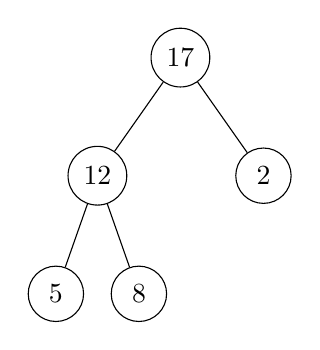
\begin{tikzpicture}
        \node {$17$}
        child {
            node {$12$}
            child { node {$5$} }
            child { node {$8$} }
        }
        child {node {$2$} };
    \end{tikzpicture}
    \hfill
    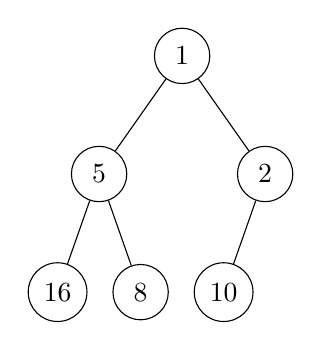
\begin{tikzpicture}
        \node {$1$}
        child {
            node {$5$}
            child { node {$16$} }
            child { node {$8$} }
        }
        child {node {$2$} 
            child { node {$10$} }
            child[missing]
        };
    \end{tikzpicture}
    \hfill
    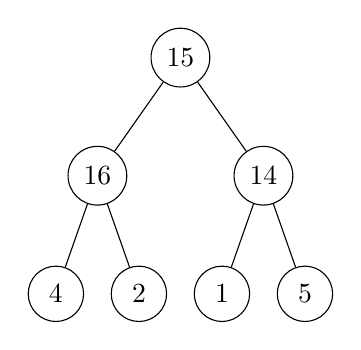
\begin{tikzpicture}
        \node {$15$}
        child {
            node {$16$}
            child { node {$4$} }
            child { node {$2$} }
        }
        child {node {$14$} 
            child { node {$1$} }
            child { node {$5$} }
        };
    \end{tikzpicture}
    \caption{A valid max-heap (left), a valid min-heap (middle), and an invalid heap (right)}
\end{figure}

Although a heap is an \bred{almost complete binary tree} \footnote{That is, the tree is completely filled on all levels except possibly the lowest, which is filled from the left up to a point. }, in practice, we usually use an array to store the data in memory. An array $H$ that represents a heap is an object with two attributes: $H$.\textit{length}, which (as usual) gives the number of elements in the array, and $H$.\textit{heap-size}, which represents how many elements in the heap are stored within array $H$. The root of the tree is $H[1]$, and given the index $i$ of a node, we can compute the indices of its parent, left child, and right child:

\begin{minipage}[t]{0.3\linewidth} \begin{itemize}
    \item \textsc{Parent}
    
    \textbf{return} $\lfloor i / 2 \rfloor$
\end{itemize} \end{minipage}
\begin{minipage}[t]{0.3\linewidth} \begin{itemize}
    \item \textsc{Left}
    
    \textbf{return} $2i$
\end{itemize} \end{minipage}
\begin{minipage}[t]{0.3\linewidth} \begin{itemize}
    \item \textsc{Right}

    \textbf{return} $2i + 1$
\end{itemize} \end{minipage}

\section{Operations}
\subsection{\textsc{Insert}}

To insert element with key $p$ into the heap $H$, 

\listu{
    \item Increment $H$.\textit{heap-size} and add a new node with key $p$ to the next available position

    \item Repeatedly swap the new item with its parent until the heap property is satisfied

    This swapping process is called \bred{bubbling up}

    \item Worst-case runtime: $\Theta(\lg n)$
}

{~~~}

For example, consider \textsc{Insert}$(H, 17)$ where $H = [16, 8, 10, 1, 5, 3]$

\begin{minipage}[t]{0.3\linewidth} \begin{center} \begin{tikzpicture} [
    every node/.style = {circle, fill=Violet, minimum size=2em}, 
    level 1/.style={sibling distance=6em}, 
    level 2/.style={sibling distance=3em}, 
    level 3/.style={sibling distance=1.5em},
    baseline=(current bounding box.north)
]
    \node {$16$} 
    child {
        node {$8$} 
        child { node {$1$} }
        child { node {$5$} }
    }
    child {
        node {$10$}
        child { node {$3$} }
        child { node [fill=MyRed] {$17$} }
    };
\end{tikzpicture} \end{center} \end{minipage}
\begin{minipage}[t]{0.3\linewidth} \begin{center} \begin{tikzpicture} [
    every node/.style = {circle, fill=Violet, minimum size=2em}, 
    level 1/.style={sibling distance=6em}, 
    level 2/.style={sibling distance=3em}, 
    level 3/.style={sibling distance=1.5em},
    baseline=(current bounding box.north)
]
    \node {$16$} 
    child {
        node {$8$} 
        child { node {$1$} }
        child { node {$5$} }
    }
    child { 
        node [fill=MyRed] (17) {$17$}
        child { node {$3$} }
        child { node (10) {$10$} }
    };

    \draw[bend left=60, dashed,latex-latex,color=MyRed]  (17) to (10);
\end{tikzpicture} \end{center} \end{minipage}
\begin{minipage}[t]{0.3\linewidth} \begin{center} \begin{tikzpicture} [
    every node/.style = {circle, fill=Violet, minimum size=2em}, 
    level 1/.style={sibling distance=6em}, 
    level 2/.style={sibling distance=3em}, 
    level 3/.style={sibling distance=1.5em},
    baseline=(current bounding box.north)
]
    \node [fill=MyRed] (17) {$17$}
    child {
        node {$8$} 
        child { node {$1$} }
        child { node {$5$} }
    }
    child { 
        node (16) {$16$}     
        child { node {$3$} }
        child { node {$10$} }
    };

    \draw[bend left=60, dashed,latex-latex,color=MyRed]  (17) to (16);
\end{tikzpicture} \end{center} \end{minipage}

\begin{algorithm}[H] \begin{algorithmic}
    \Procedure{Max-Heap-Insert}{$H$, $p$}
        \State $i \gets H.\textit{heap-size} \gets H.\textit{heap-size} + 1$
        \State $H[i] = p$
        \While{$\textsc{Parent}(i) > 0$ \textbf{and} $H[i] > H[\textsc{Parent}(i)]$}
            \State swap $H[i]$ with $H[\textsc{Parent}[i]]$
            \State $i \gets \textsc{Parent}(i)$
        \EndWhile
    \EndProcedure
\end{algorithmic} \end{algorithm}

\subsection{\textsc{Find-Max}}

To find the maximum key in the heap $H$, 

\listu{
    \item Simply return the item in the root

    \item Worst-case runtime: $\Theta(1)$
}

\begin{center} \begin{tikzpicture} [
    every node/.style = {circle, fill=Violet, minimum size=2em}, 
    level 1/.style={sibling distance=6em}, 
    level 2/.style={sibling distance=3em}, 
    level 3/.style={sibling distance=1.5em},
    baseline=(current bounding box.north)
]
    \node (root) {$17$}
    child {
        node {$8$} 
        child { node {$1$} }
        child { node {$5$} }
    }
    child { 
        node (16) {$16$}     
        child { node {$3$} }
        child { node {$10$} }
    };
    
    \draw[bend left=30, dashed, -latex, color=MyRed] (-1.25,0.5) to (-0.25,0.5);
\end{tikzpicture} \end{center}

\begin{algorithm}[H] \begin{algorithmic}[1]
    \Procedure{Find-Max}{$H$}
        \State \Return $H[1]$
    \EndProcedure
\end{algorithmic} \end{algorithm}

\subsection{\textsc{Extract-Max}}

\listu {
    \item Save the item from the root in a temporary variable
    \item Replace the root with the rightmost item in the lowest level of the tree and decrement $H$.\textit{heap-size}
    \item Repeatedly swap the item we moved with its largest child until the heap property is restored. This swapping process is called \bred{bubble down}.
    \item Worst-case runtime: $\Theta(\lg n)$
}

\begin{minipage}[t]{0.32\linewidth} \begin{center} \begin{tikzpicture} [
    every node/.style = {circle, fill=Violet, minimum size=2em}, 
    level 1/.style={sibling distance=6em}, 
    level 2/.style={sibling distance=3em}, 
    level 3/.style={sibling distance=1.5em},
    baseline=(current bounding box.north)
]
    \node[fill=MyRed] (root) {$17$}
    child {
        node {$8$} 
        child { node {$1$} }
        child { node {$5$} }
    }
    child { 
        node (16) {$16$}     
        child { node {$3$} }
        child { node {$10$} }
    };

    \node[left of=root, node distance=2cm] (17) {$17$};
    
    \draw[dashed, -latex, color=MyRed] (root) to (17);
    \draw[bend right=60, dashed, -latex, color=MyRed] (10) to (root);
\end{tikzpicture} \end{center} \end{minipage}
\begin{minipage}[t]{0.32\linewidth} \begin{center} \begin{tikzpicture} [
    every node/.style = {circle, fill=Violet, minimum size=2em}, 
    level 1/.style={sibling distance=6em}, 
    level 2/.style={sibling distance=3em}, 
    level 3/.style={sibling distance=1.5em},
    baseline=(current bounding box.north)
]
    \node[fill=MyRed] (root) {$10$}
    child {
        node {$8$} 
        child { node {$1$} }
        child { node {$5$} }
    }
    child { 
        node (16) {$16$}     
        child { node {$3$} }
        child[missing]
    };
    
    \draw[bend left=60, dashed, latex-latex, color=MyRed] (root) to (16);
\end{tikzpicture} \end{center} \end{minipage}
\begin{minipage}[t]{0.32\linewidth} \begin{center} \begin{tikzpicture} [
    every node/.style = {circle, fill=Violet, minimum size=2em}, 
    level 1/.style={sibling distance=6em}, 
    level 2/.style={sibling distance=3em}, 
    level 3/.style={sibling distance=1.5em},
    baseline=(current bounding box.north)
]
    \node (root) {$16$}
    child {
        node {$8$} 
        child { node {$1$} }
        child { node {$5$} }
    }
    child { 
        node[fill=MyRed] (10) {$10$}     
        child { node {$3$} }
        child[missing]
    };
    
    \draw[bend left=60, dashed, latex-latex, color=MyRed] (root) to (16);
\end{tikzpicture} \end{center} \end{minipage}

\begin{algorithm}[H] \begin{algorithmic}[1]
    \Procedure{Extract-Max}{$H$}
        \State $\textit{max} \gets H[1]$

        \State $H[1] \gets H[H.\textit{heap-size}]$

        \State $H.\textit{heap-size} \gets H.\textit{heap-size} - 1$

        \State \textsc{Max-Heapify}$(H, 1)$

        \State \textbf{return} \textit{max}
    \EndProcedure
\end{algorithmic} \end{algorithm}

\begin{algorithm}[H] \begin{algorithmic}[1]
    \Procedure{Max-Heapify}{$H$, $i$}
        \State $l \gets \textsc{Left}(i)$
        \State $r \gets \textsc{Right}(i)$

        \If {$l \leq H.\textit{heap-size}$ \textbf{and} $H[l] > H[i]$}
            \State $\textit{largest} \gets l$
        \Else
            \State $\textit{largest} \gets i$
        \EndIf

        \If {$r \leq H.\textit{heap-size}$ \textbf{and} $H[r] > H[\textit{largest}]$}
            \State $\textit{largest} \gets r$
        \EndIf

        \If {$\textit{largest} \neq i$}
            \State swap $H[i]$ with $H[\textit{largest}]$
            \State \textsc{Max-Heapify}$(H, \textit{largest})$
        \EndIf
    \EndProcedure
\end{algorithmic} \end{algorithm}

\subsection{\textsc{Build-Max-Heap}}

\listu {
    \item Takes an array $A$ of length $n$ and builds a max-heap $H$ from it.
    \item Worst-case runtime: $\Theta(n)$
}

\begin{algorithm}[H] \begin{algorithmic}[1]
    \Procedure{Build-Max-Heap}{$A$}
        \State $H.\textit{heap-size} \gets A.\textit{length}$
        \For {$i = \lfloor \frac{A.\textit{length}}{2} \rfloor$ \textbf{downto} $1$}
            \State \textsc{Max-Heapify}$(H, i)$
        \EndFor
    \EndProcedure
\end{algorithmic} \end{algorithm}